\section{Descrizione delle classi}
\subsection{Gerarchia degli utenti}

\begin{figure}[h]
  \caption{Struttura logica della gerarchia degli utenti}
  \centering
  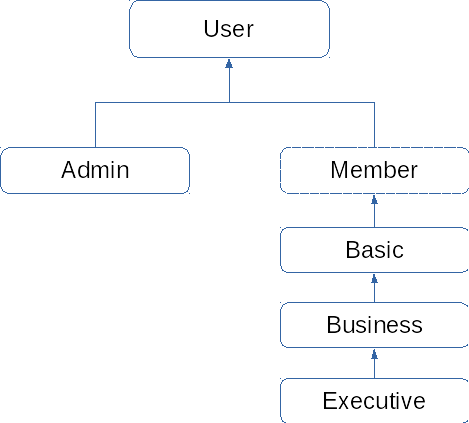
\includegraphics[width=8cm,height=8cm,keepaspectratio]{res/userclass}
\end{figure}

Alla base di tutta la gerarchia degli utenti � presente la classe ``Users''.
Questa \`e una classe virtuale, che contiene informazione di base,
come il tipo di account in uso, il Database a cui appartiene e la sua
validit\`a. Dato che logicamente non ha senso che esista un User, essa non
� istanziabile. \newline
Derivato a User c'\`e Admin, che � una classe istanziabile e concreta.
Essa implementa le funzionalit\`a dell'amministratore, come il metodo
di ricerca, il cambiamento di tipo di un Membro, la sua aggiunta e la sua
cancellazione. \newline

Derivata da User c'\`e anche la classe Member, virtuale pura. Essa pone le
basi per tutti le tipologie di iscritti a LinQedIn. Qui � presente il metodo
search da implementare per ogni classe. Member implementa gi� la scrittura
e la lettura delle informazioni dal database xml per ogni tipologia di
iscritto. Basic, Business, Executive sono classi derivate che implementano
la ricerca sul Database.

\subsubsection{Classi contenute in Member}

Member contiene diverse classi, a loro volta formate da pi\`u classi o
derivate, essa \`e formata da un \textit{Profile} e da
\textit{Friendships}.

\paragraph*{Profile} \`e una classe che contiene le informazioni
personali e la carriera dell'iscritto, ingloba tramite una relazione
\textit{has-a} le classi \textit{Personal} ed \textit{Experiences}. \newline
Personal contiene a sua volta \textit{Bio, Hobby, Interests}. \`E da
notare che \textit{Hobby, Interests} e \textit{Experiences} derivano da
classi contenitori. Questa scelta di creare dei wrapper \`e dovuta alla
maggiore estendibilit\`a del codice: se un domani si volesse cambiare
contenitore, le modifiche andrebbero eseguite solo in quelle classi.

\paragraph*{Friendships} deriva da un contanier \textit{vector} e si occupa
di salvare le amicizie di ogni Membro. L'amicizia viene salvata tramite il
nickName, che \`e univoco per tutto il Database.

\subsection{Gerarchia degli SmartPointer}

\begin{figure}[h]
  \caption{Struttura logica della gerarchia dei puntatori smart}
  \centering
  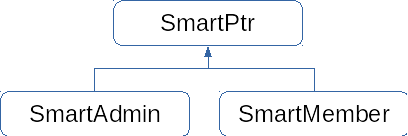
\includegraphics[width=8cm,height=8cm,keepaspectratio]{res/smartptrclass}
\end{figure}

Nonostante la gestione della memoria condivisa non sia stato un problema
data la natura implementativa del progetto, \`e stato deciso comunque
di utilizzare puntatori smart. SmartPtr \`e una classe base con il
costruttore dichiarato protected, questo per impedirne una sua
istanziazione tranne che per le classi derivate da essa: avere una classe
base comune a tutti i smartPtr permette di aggiungere funzionalit\`a a tutte le classi derivate, e di introdurre metodi virtuali o puri. \textit{SmartAdmin} e \textit{SmartMember} gestiscono la condivisione in memoria
rispettivamente di Admin e Member, utilizzando il reference counting.

\subsection{Gerarchia della gestione degli User}

\begin{figure}[h]
  \caption{Struttura logica della gerarchia per la gestione degli User}
  \centering
  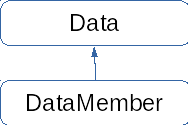
\includegraphics[width=3cm,height=3cm,keepaspectratio]{res/dataclass}
\end{figure}

Come scelta progettuale, si \`e deciso di non tenere la lista degli utenti
direttamente sul Database, ma di creare una gerarchia di classi per la
gestione di essi che poi verranno gestite a loro volta dal Database.
Questo permette una pi\`u facile gestione degli utenti (attualmente solo
Membri, ma potrebbero esserci altre tipologie).
La gerarchia ricalca la stessa struttura data per gli smart pointer e per
gli user.

\subsection{Database e gerarchia}

